\documentclass[oneside, 11pt]{article}

\usepackage[T1]{fontenc}
\usepackage[utf8]{inputenc}
\usepackage[english]{babel}
\usepackage{enumerate}
\usepackage{isotope}


\usepackage{fouriernc}
\usepackage[detect-all, binary-units, separate-uncertainty=true,
            per-mode=symbol, retain-explicit-plus, retain-unity-mantissa=false]{siunitx}

\usepackage{setspace}
\setstretch{1.2}

\setlength{\parskip}{\smallskipamount}
\setlength{\parindent}{0pt}

\usepackage[headheight=14pt]{geometry}
\geometry{marginparwidth=0.5cm, verbose, a4paper, tmargin=3cm, bmargin=3cm,
          lmargin=2cm, rmargin=2cm}

\usepackage{float}

\usepackage[fleqn]{amsmath}
\numberwithin{equation}{section}
\numberwithin{figure}{section}

\usepackage{graphicx}
\graphicspath{{images/}{../../../images/}}

\usepackage{tikz}
\usetikzlibrary{shapes}
\usetikzlibrary{plotmarks}

\newcounter{Exercise}
\setcounter{Exercise}{1}
\usepackage{xcolor}
\definecolor{shadecolor}{gray}{0.9}
\usepackage{framed}
\usepackage{caption}

\usepackage{url}


\usepackage{fancyhdr}
\pagestyle{fancy}
\fancyhf{}
\rhead{\thepage}
\renewcommand{\footrulewidth}{0pt}
\renewcommand{\headrulewidth}{0pt}

\fancypagestyle{firststyle}
{
    \fancyhf{}
    \rhead{\thepage}
    \cfoot{\includegraphics[height=30pt]{HiSPARClogo}}
    \rfoot{\includegraphics[height=25pt]{CCbysa}}
    \lfoot{
\includegraphics[height=30pt]{NIKHEFlogo}}
    \renewcommand{\footskip}{50pt}
    \renewcommand{\footrulewidth}{0.1pt}
    \renewcommand{\headrulewidth}{0pt}
}

\newcommand{\figref}[1]{Figuur~\ref{#1}}

\newcommand{\hisparc}{\textsmaller{HiSPARC}\xspace}
\newcommand{\kascade}{\textsmaller{KASCADE}\xspace}
\newcommand{\sapphire}{\textsmaller{SAPPHiRE}\xspace}
\newcommand{\jsparc}{\textsmaller{jSparc}\xspace}
\newcommand{\hdf}{\textsmaller{HDF5}\xspace}
\newcommand{\aires}{\textsmaller{AIRES}\xspace}
\newcommand{\csv}{\textsmaller{CSV}\xspace}
\newcommand{\python}{\textsmaller{PYTHON}\xspace}
\newcommand{\corsika}{\textsmaller{CORSIKA}\xspace}
\newcommand{\labview}{\textsmaller{LabVIEW}\xspace}
\newcommand{\daq}{\textsmaller{DAQ}\xspace}
\newcommand{\adc}{\textsmaller{ADC}\xspace}
\newcommand{\hi}{\textsc{h i}\xspace}
\newcommand{\hii}{\textsc{h ii}\xspace}
\newcommand{\mip}{\textsmaller{MIP}\xspace}
\newcommand{\hisparcii}{\textsmaller{HiSPARC II}\xspace}
\newcommand{\hisparciii}{\textsmaller{HiSPARC III}\xspace}

\DeclareSIUnit{\electronvolt}{\ensuremath{\mathrm{e\!\!\:V}}}

\DeclareSIUnit{\unitsigma}{\ensuremath{\sigma}}
\DeclareSIUnit{\mip}{\textsmaller{MIP}}
\DeclareSIUnit{\adc}{\textsmaller{ADC}}

\DeclareSIUnit{\gauss}{G}
\DeclareSIUnit{\parsec}{pc}
\DeclareSIUnit{\year}{yr}





%document details
\author{Koos Kortland \\ translated and adapted by K. Schadenberg}
\date{}
\title{Air Showers}


\begin{document}
\maketitle

\section{Introduction}
The HiSPARC project tries to measure air showers; the product of high energetic particles hitting our atmosphere. In this module we will take a first look at what an air shower is and its important properties.

Throughout our Galaxy there is a continuous flow of high energetic charged particles. The flux of this flow is about one hundred thousand particles per square meter per second. Most of these particles are protons 85\%, alpha particles (helium nuclei) 12\%, and electrons 2\%. The remainder are heavier nuclei such as carbon and oxygen. Stars like our Sun our one of the many sources of these particles. But more violent processes, such as supernovae, are able to sling these particles into space at great velocities.

\section{Energy Spectrum}
The energy of the particles colliding with the Earth's atmosphere is shown in figure~\ref{fig:spectrum}. This graph makes clear that the number of particles rapidly decreases with increasing energy, especially at the highest energies (above $10^{15}$~eV). Here there is a small bend in the line. This bend is called the knee, below the knee the flux decreases even more rapidly then above.

\begin{figure}\begin{center}
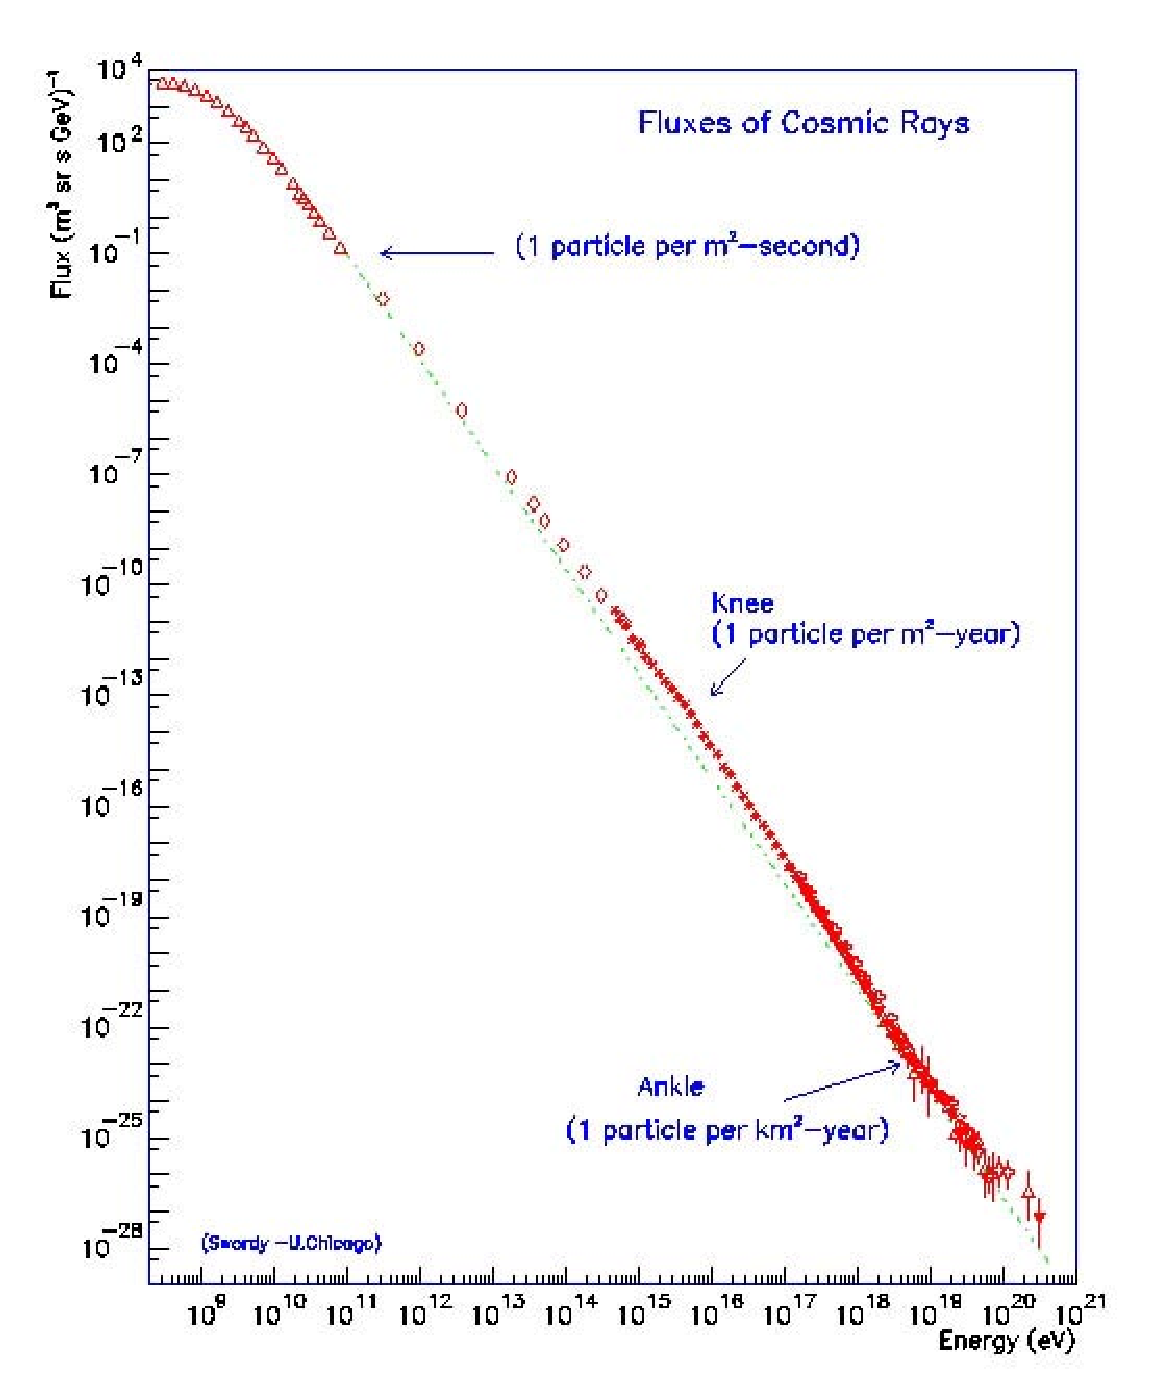
\includegraphics[scale=0.6]{spectrum.eps}%
\caption{The energy spectrum of charged cosmic particles. The flux, number of particles per unit area and unit time, is dependent on the energy (horizontal axis).}\label{fig:spectrum}
\end{center}\end{figure}

Particles with energies above $10^{15}$~eV are able to escape the Milky Way, while less energetic particles are trapped. This accounts for the faster decrease in particles above the knee. The particles are trapped by the magnetic field of the Milky Way. Although very weak, it stretches out across the entire galaxy making the charged particles spin around inside. Because of the circling motion around the galaxy we cannot locate the source of these particles.

Particles with higher energies can escape our galaxy, this also means that particles from other galaxies can travel to ours. After a long journey through intergalactic space they might end up at our doorstep, the Earth's atmosphere. Because these particles are influenced (deflected) less by the magnetic fields present all across the universe we might be able to discover their origins. However, the flux of these particles at the outer layers of the atmosphere is less than one particles per square meter per year.

We do not expect to see any particles with energies in excess of $10^{19}$~eV because these particles would quickly lose energy while interacting with the Cosmic Microwave Background radiation (CMB). But if you look carefully at figure~\ref{fig:spectrum} you see that there are actually a few particles with this tremendous amount of energy.

\section{Air Showers}
During its flight though the atmosphere a cosmic ray particle has a high probability of colliding with a nitrogen or oxygen nucleus, the principal components of our atmosphere. A collision only happens when the interaction between the cosmic ray and the nucleus is strong enough. This is the case if the the (primary) cosmic ray is a high energetic photon or charged nucleus that comes close enough to the nuclei present in the atmosphere. A neutrino on the other hand does not leave behind a trace when travelling through the air.

The result of the initial collision is the creation of new (secondary) particles. These particles have a lower energy than the primary particle but are still highly energetic. These secondary particles can also collide with a nitrogen or oxygen nucleus, again producing new, but less energetic, particles. Collisions followed by collisions followed by collisions create large scale events we call air showers. It is as though there is a shower of particles coming towards the surface of the Earth after a cosmic ray hit our atmosphere. In figure~\ref{fig:shower} shows such an air shower.

\begin{figure}\begin{center}
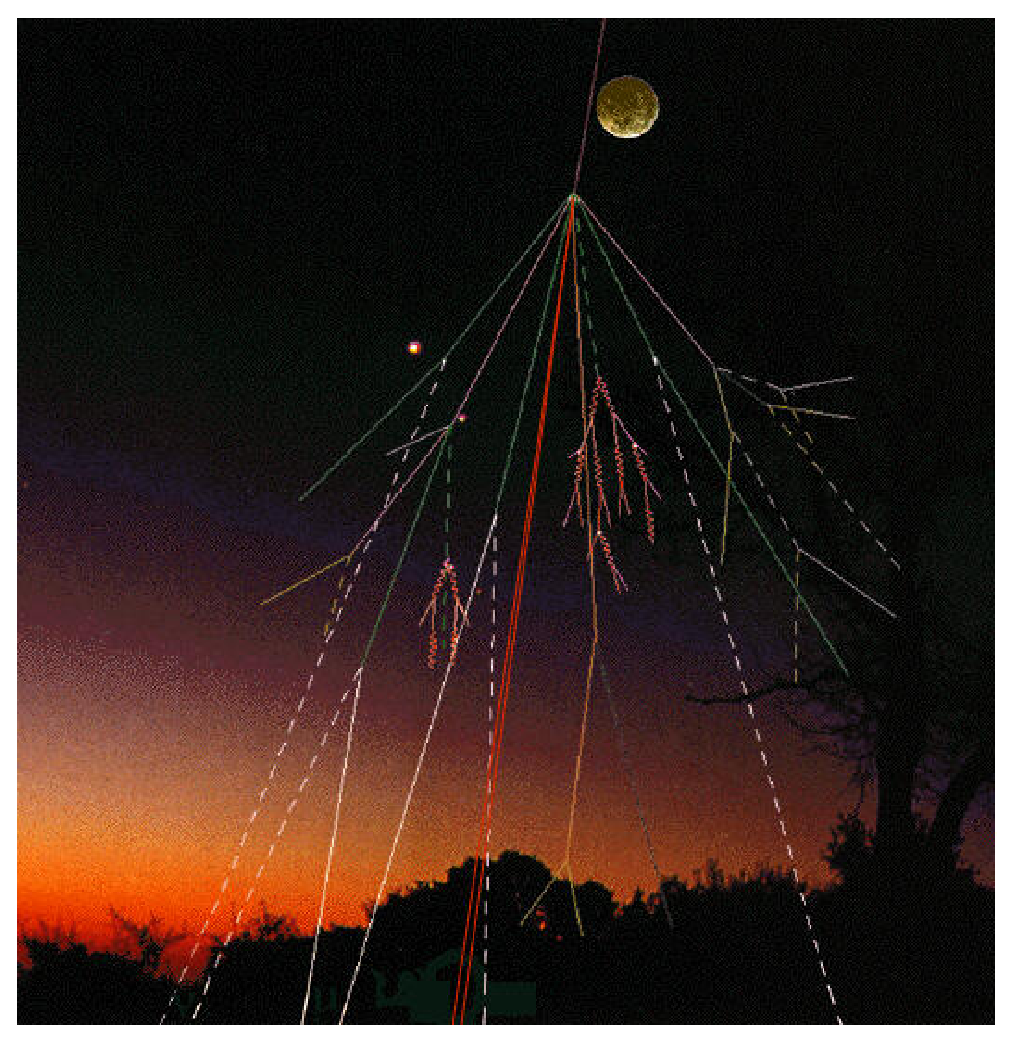
\includegraphics[scale=0.38]{shower.eps}%
\caption{Schematic representation of a part of an air shower. The primary particle creates a limited number of secondary particles of which a few reach the Earth's surface.}\label{fig:shower}
\end{center}\end{figure}

This figure shows that not all the particles reach the surface of the Earth. Depending on the altitude of the first collision, the secondary particles must travel a distance of 10 to 40~kilometres. Only if the primary particle had enough energy, more than 5~GeV, are the secondary particles able to reach the surface. On the following website you can see a number of realistic simulations of different air showers:\\
\url{th.physik.uni-frankfurt.de/\~drescher/CASSIM/}

\begin{shaded}
\textbf{Exercise \theExercise \stepcounter{Exercise}} : In simulations of air showers charged particles move between collisions along a straight path. However, these particles are inside the magnetic field of the Earth and are therefore subjected to Lorentz forces possibly influencing their trajectory. The question arises whether we should take these effects into account in our simulations.
\begin{enumerate}[-]
\item Shows, using derivations of known equations, that for a charged particle with mass $m$ and charge $q$ moving with speed $v$ through a homogeneous magnetic field $B$ the following equation holds:
\begin{equation}
B \cdot q \cdot r = m \cdot v = p
\end{equation}
with $r$ the radius of curvature of the particle's orbit and $p$ its momentum.
\item Momentum is a relativistic correct quantity so we need not worry about mass changing with velocity.\footnotemark~Show that a muon with an energy $E$ of 1~GeV has a momentum $p=1~\frac{\mbox{GeV}}{c}$.
\item Calculate the radius of curvature of the orbit of a muon with momentum $p=1~\frac{\mbox{GeV}}{c}$ inside the Earth's magnetic field (roughly 50~$\mu$T).
\item What is your final conclusion? When simulating charged particles inside an air shower, do we need to take into account the deflection caused by the magnetic field of the Earth? Explain why or why not?
\end{enumerate}\end{shaded}
\footnotetext{See the modules `Muon decay' and `Relativity' for more details.}

\section{Types of Showers}
Below we we briefly describe a few of the characteristic of air showers: how they form, their composition, and how they spread out through the atmosphere. We will focus on the most energetic primary particles because they are of the most interest to the HiSPARC project. We will use this to answer the reverse question: If we measure certain particles (type, density, and energy) on the Earth surface, can we reconstruct the shower and tell what kind of particle (type, energy, and direction) started the shower?

To do this we must first take a look at the different types of showers: electromagnetic and hadronic showers.

\subsection{Electromagnetic Showers}
The starting point of an air shower, the primary cosmic particle, can be a photon or charged particle. Charged particles have stronger interactions with the atomic nuclei inside the atmosphere than photons. As a consequence photons have, on average, their first collision deeper inside the atmosphere, i.e. closer to the surface of the Earth than protons. Heavier nuclei will have their first collision sooner, higher up in the atmosphere than lighter nuclei.

What type of particle initiates the shower also dictates the composition of secondary particles inside the air shower. Photons only have the electromagnetic force to interact with other matter. As a result photons can only create pairs of particles with their anti-particles, mostly electrons and positrons. These particles in turn can produce new photons, for instance when they move through the electrical field of an atomic nucleus or when the positron annihilates when it encounters an electron.

The main constituents of showers started by photons (gamma rays) are photons, electrons, and positrons. We therefore call them electromagnetic showers. Muons are also present in these showers. But because the muon is roughly 200 times as heavy as the electron it takes a lot more energy to create a $\mu^+$ $\mu^-$ pair than it takes to create an $e^+$ $e^-$ pair.

\subsection{Hadronic Showers}
A high energetic proton entering the atmosphere will, like the photon, interact with other matter via the electromagnetic force. But a more important way of interacting is via the strong (nuclear) force, the force exerted by quarks onto other quarks. Because of the energies involved in this type of interaction, collision, we can say that they are collisions between the individual components of the proton (quarks and gluons) and the nucleons present in the atmosphere (protons and neutrons inside the nitrogen and oxygen atoms).

During these interactions new nucleon particles are created using the strong force. A large part of these new particles are mesons, bound quark anti-quark pairs. The lightest and therefore most frequently created meson is the pion. There are three different pions: $\pi^+$, $\pi^-$, and $\pi^0$. These particle are not stable and after a short time they decay into other particles. The average lifetime of a charged pion is $2.6 \cdot 10^{-8}$~s after which it decays into a muon, with the same charge, and an (anti) neutrino. The neutral pion decays even faster, after $0.8 \cdot 10^{-16}$~s, into two photons.

Because a large number of hadrons are created in shower initiated by charged nuclei we call them hadronic showers. Inside a hadronic shower, a neutral $\pi^0$ meson with an energy of 10~GeV will travel an average distance of 2~$\mu$m before it decays into photons. A charged $\pi^-$ or $\pi^+$ meson's lifetime is $3 \cdot 10^8$ times as long and can, with the same energy, travel a distance of 600~m before decaying into a muon. Most pions will therefore never reach the Earth's surface. But because of pion decay large numbers of muons are created inside hadronic showers. These are able to reach the surface. With an average lifetime of $2.2 \cdot 10^{-6}$~s and having roughly the same energy as the pion (the neutrino only takes away a small portion of the energy), in this case 10~GeV, they can travel 5 to 10~kilometres before decaying. Moreover muons are capable of penetrating large amounts of matter; they only lose small amounts of energy during collisions/interactions.

Protons and neutrons are also capable of reaching the Earth's surface. Because of their large mass, ten times as large as a muon, they are only created infrequently inside a hadronic shower and stay close to the centre of the shower. Detectors placed on Earth will therefore mostly measure muons, electrons, and photons.

\section{Characteristic Depth}
Inelastic collisions create large numbers of new particles during the creation of an air shower. Each new particle carries a part of the primary particles energy. The collisions continue to create new particles until the energy per particle is too low for the creation of new particles. Up to that point the particle density inside the shower increases. When the energy falls below this critical level the particles are only scattered and the particle density decreases. Figure~\ref{fig:shower_density} shows this behaviour in a graph as well as the dominant particles at each level. The altitude at which the maximum particle density is achieved is called the characteristic depth $x_{\mbox{max}}$ (see figure~\ref{fig:x_max}).

\begin{figure}\begin{center}
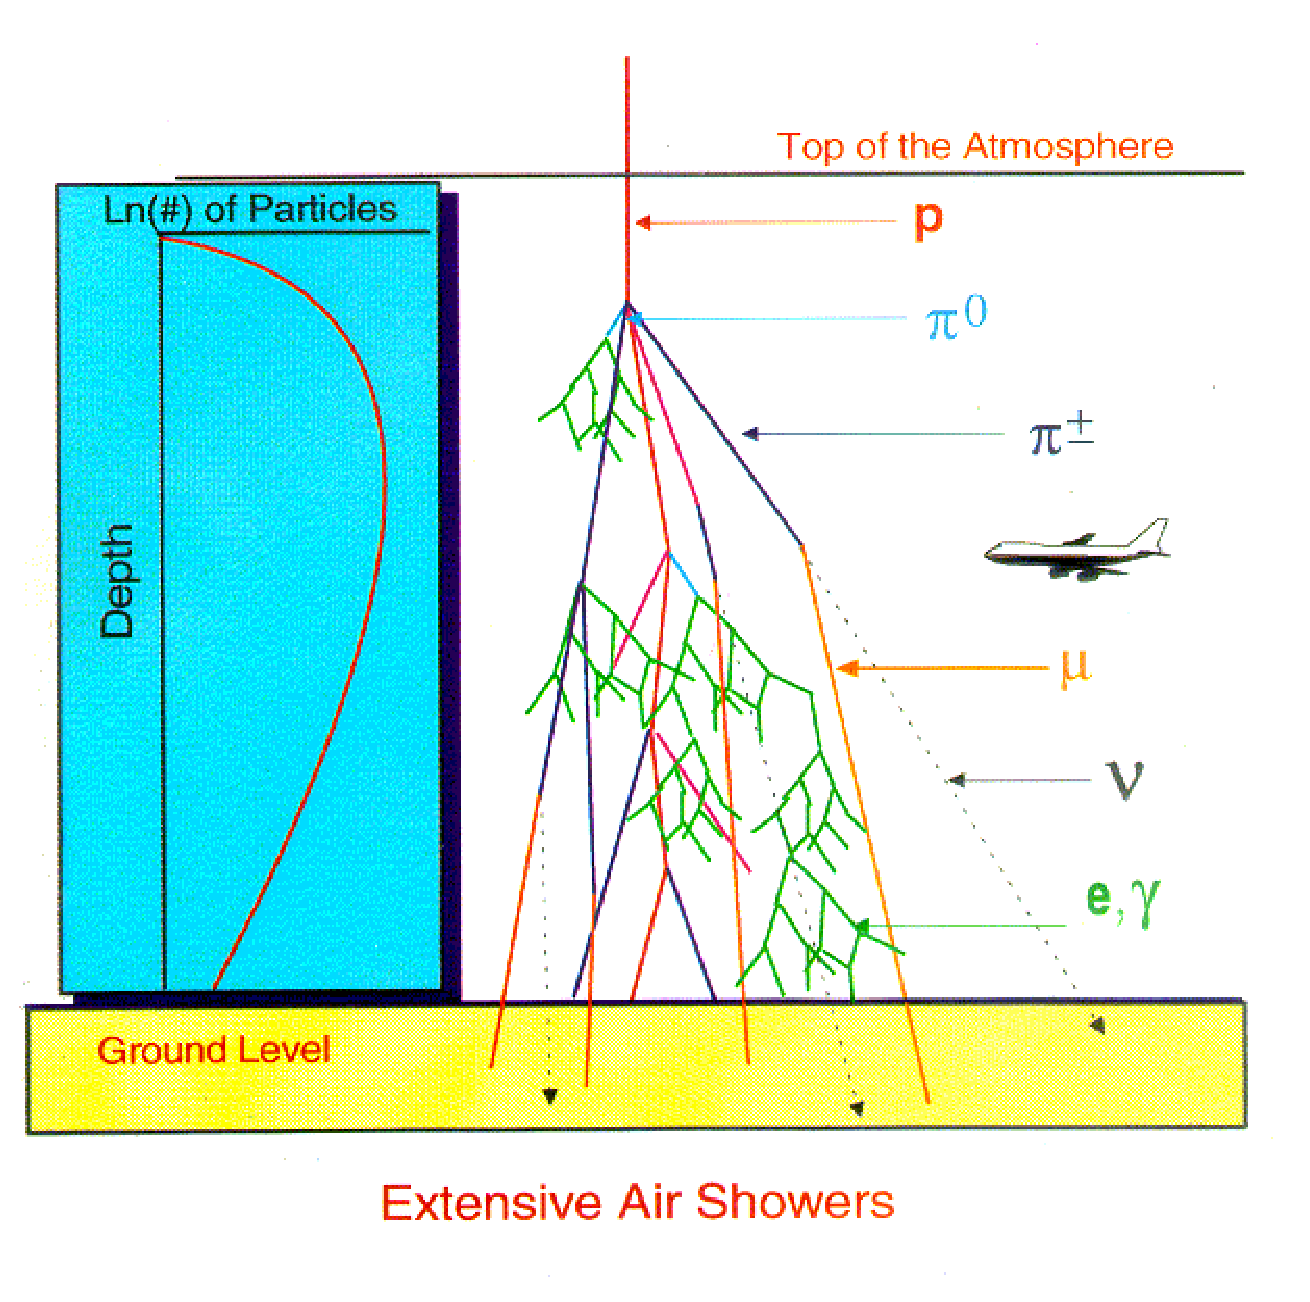
\includegraphics[scale=0.45]{shower_density.eps}%
\caption{The development of an air shower, on the left hand side the particle density as a function of depth inside the atmosphere.}\label{fig:shower_density}
\end{center}\end{figure}

\begin{figure}\begin{center}
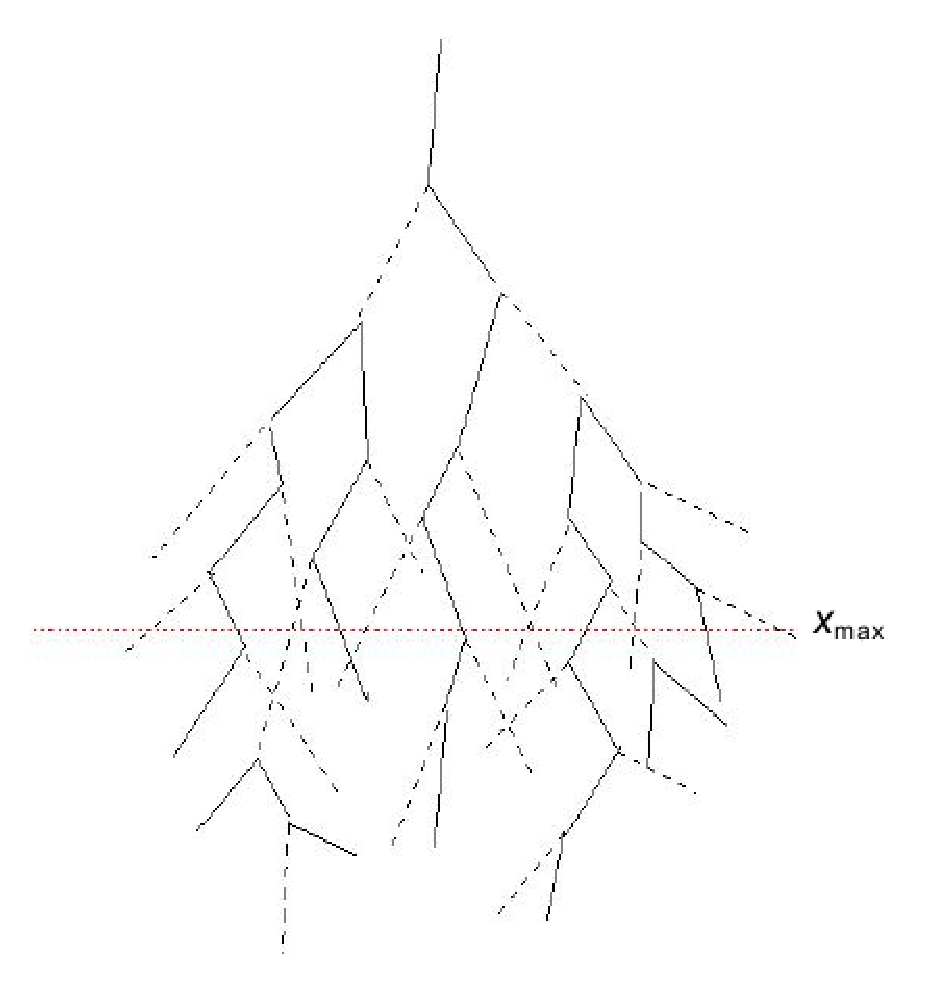
\includegraphics[scale=0.5]{x_max.eps}%
\caption{Schematic representation of the development of an air shower. The highest particle density is at a depth $x_{\mbox{max}}$ inside the atmosphere, measured from the starting point of the shower.}\label{fig:x_max}
\end{center}\end{figure}

The total depth of the shower, or reach of the shower, and the characteristic depth not only depend on the primary particle's energy and the depth of the first collision, but also on the atmospheric conditions. The number of collisions or distance before collision for each particle depends directly on the product between the chance of collision per target (chance to hit a single particle) and the number of possible targets. The first factor only depends on the types of particles involved in the collision (a collision between a photon and a nucleon is different from a collision between a proton and a nucleon).

The second factor is directly proportional to the particle density along the trajectory of the shower. This density is influenced by amongst others; the height, (ambient) air pressure, and temperature. It is therefore customary not to report the progress of the shower in metres but with respect to the amount of matter the shower has passed though. This quantity is reported in grams per centimetre squared (g/cm$^2$). At sea level there is a column of mass 1030 g/cm$^2$ `thick' above us. Only the most energetic particles are able to create showers with $x_{\mbox{max}}$ at this level.

\section{Tracking Showers}
The development of showers can be tracked using the light which is emitted when the molecules in the air are exited by the passing particles inside the shower. The intensity of the light is a good measure for the total flux of particles (predominantely electrons) at all levels of the shower. However, this light is very dim making it only visible on the clearest moonless nights.

The Fly's Eye / HiRes experiment in the desert of Utah (USA) was designed to measure the light produced by air showers with great detail. Figure~\ref{fig:HiRES} shows one of the measurement sites of this experiment and figure~\ref{fig:profile} shows the electron density profile in a shower created by a $0.8 \cdot 10^{18}$~eV primary particle as determined by the HiRes experiment.

\begin{figure}\begin{center}
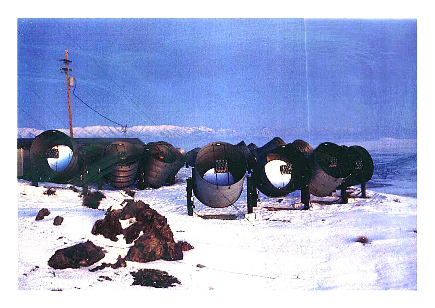
\includegraphics[scale=1]{HiRES.eps}%
\caption{The Fly's Eye / HiRes experiment in de desert of Utah (USA).}\label{fig:HiRES}
\end{center}\end{figure}

\begin{figure}\begin{center}
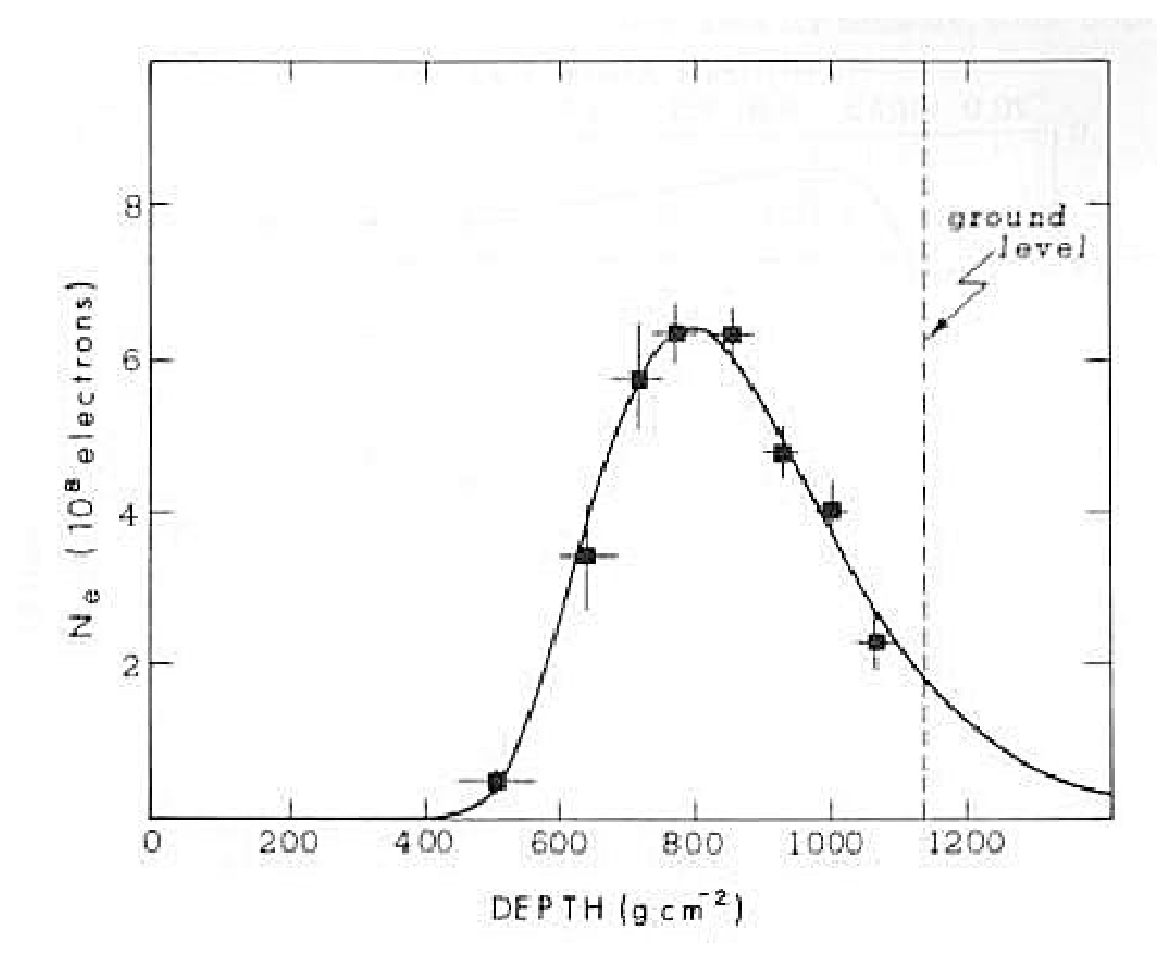
\includegraphics[scale=0.5]{profile.eps}%
\caption{The number of electrons as function of the (horizontal) depth in air showers initiated by $0.8 \cdot 10^{18}$~eV primary particles.}\label{fig:profile}
\end{center}\end{figure}

A different way of directly measuring the particle density uses low frequency radio waves. These radio waves are generated by the electrical current of charged particles inside a shower. The LOFAR radio telescope which is spread out across main land Europe and parts of the UK night be able to `hear' these radio signals.

More information about these two experiments can be found at:\\
\url{hires.physics.utah.edu} \\
\url{lofar.org}

\section{Shower Profiles}
Lets take another look at figure~\ref{fig:profile}. The vertical profile of an air shower is different for the two types of shower; electromagnetic and hadronic. Figure~\ref{fig:profile2} also shows the profile of electrons but now for three different primary particles and at a slightly higher energy. This graph is the result of a simulation and not of a direct measurement like figure~\ref{fig:profile}. Figure~\ref{fig:profile2} clearly shows the differences between the primary particles and the influence it has on $x_{\mbox{max}}$. 

\begin{figure}\begin{center}
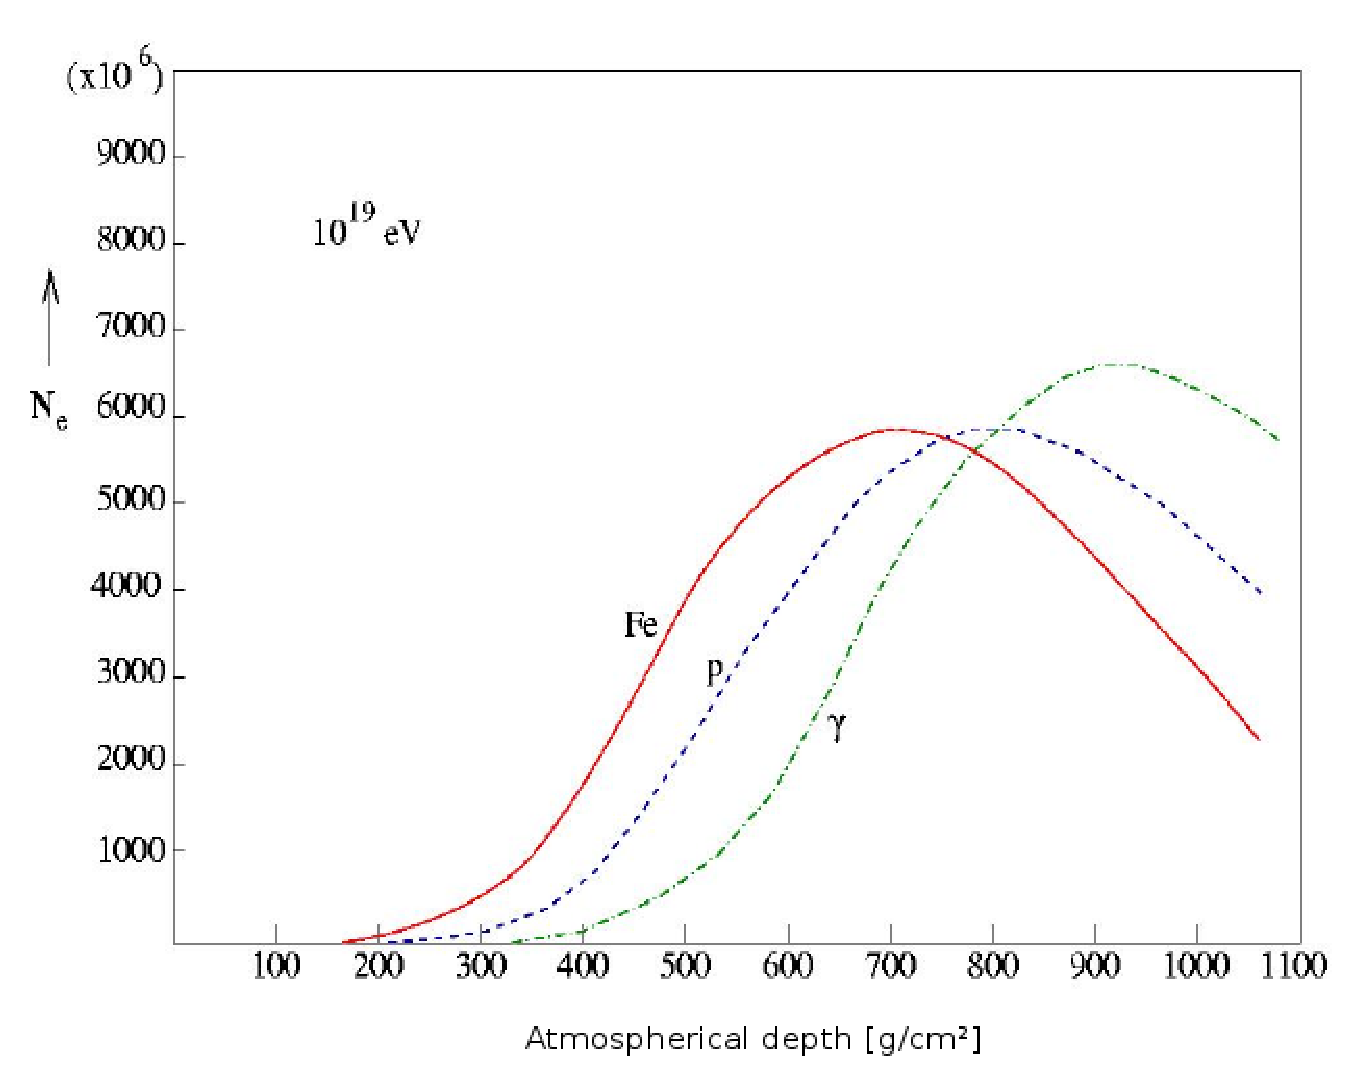
\includegraphics[scale=0.5]{profile2.eps}%
\caption{The number of electrons as function of shower depth for different primary particles, all with an energy of $10^{19}$~eV: iron nucleus (Fe), proton (p), and photon ($\gamma$).}\label{fig:profile2}
\end{center}\end{figure}

We can also look at the horizontal profile of showers: figure~\ref{fig:profile3}. This profile shows the number of particles as a function of the distance to the shower core axis measured in a plane perpendicular to this axis. Figure~\ref{fig:profile3} not only shows the density of electrons, but also the densities of photons and muons. 

\begin{figure}\begin{center}
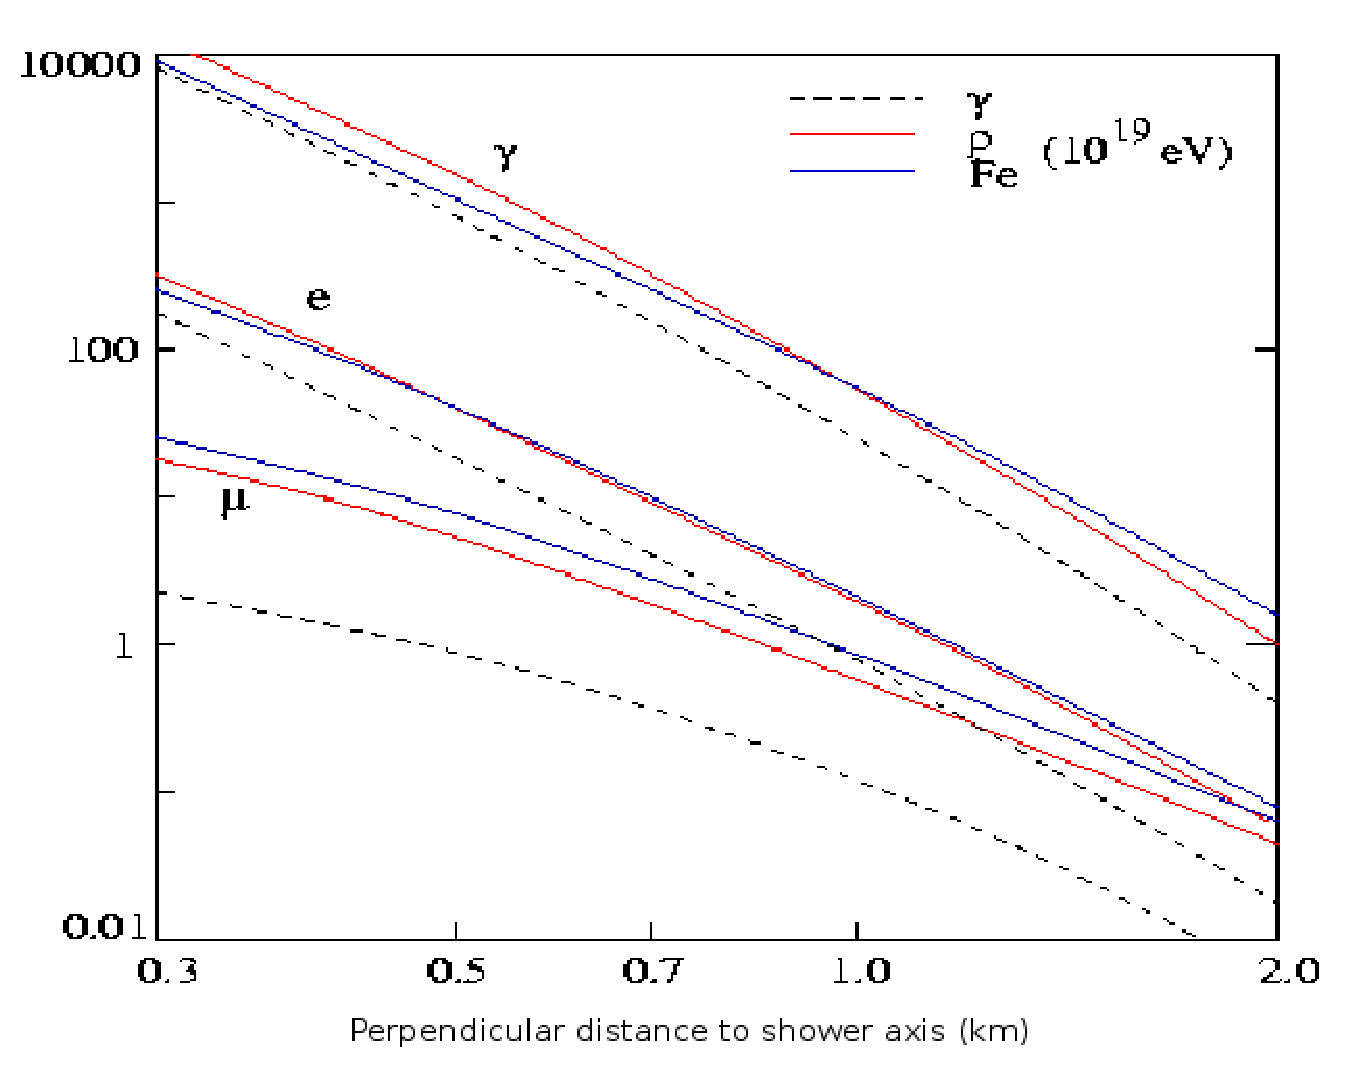
\includegraphics[scale=0.5]{profile3.eps}%
\caption{The number of photons ($\gamma$), electrons (e), and muons ($\mu$) at a depth of 860~g/cm$^2$ as functions of the distance to the shower core. Simulated for different primary particles (Fe, p, and $\gamma$), all with an initial energy of $10^{19}$~eV. }\label{fig:profile3}
\end{center}\end{figure}

\begin{shaded}
\textbf{Exercise \theExercise \stepcounter{Exercise}} : Figures~\ref{fig:profile2} and \ref{fig:profile2} show two different types of shower profiles, vertical and horizontal, for three different primary particles.
\begin{enumerate}[-]
\item Explain the (global) shape of both types of shower profiles depicted in figures~\ref{fig:profile2} and \ref{fig:profile2}.
\item What is, according to figure~\ref{fig:profile2}, the most important difference between an electromagnetic and hadronic shower when looking at the particle densities near the surface of the Earth. Does this agree with the description of these types of showers given earlier in this text?
\item What do you need to measure at ground level to tell if a shower is created by a photon or by a atomic nucleus?
\end{enumerate}\end{shaded}

\begin{shaded}
\textbf{Exercise \theExercise \stepcounter{Exercise}} : A group of particle detectors are placed in an area, like the HiSPARC setup. They can measure the number of particles inside an air shower passing by and the exact time at which this happens. How can this data be used to determine the energy and direction of the primary cosmic ray?\end{shaded}

\section{Energy of an Air Shower}
As mentioned earlier the number of photons and electrons inside an air shower is much larger than the number of muons. This difference is greatest in the electromagnetic showers. Both photons and electrons are stable particles but quickly lose their energy in elastic or inelastic collisions inside the atmosphere. As a consequence, in hadronic showers the largest deposition of energy at ground level is done by muons, even though there are many more photons and electrons. This is shown in figure~\ref{fig:profile_flux}. The same profile would look very different for electromagnetic showers because the number of muons is much lower, roughly a factor 10.

\begin{figure}\begin{center}
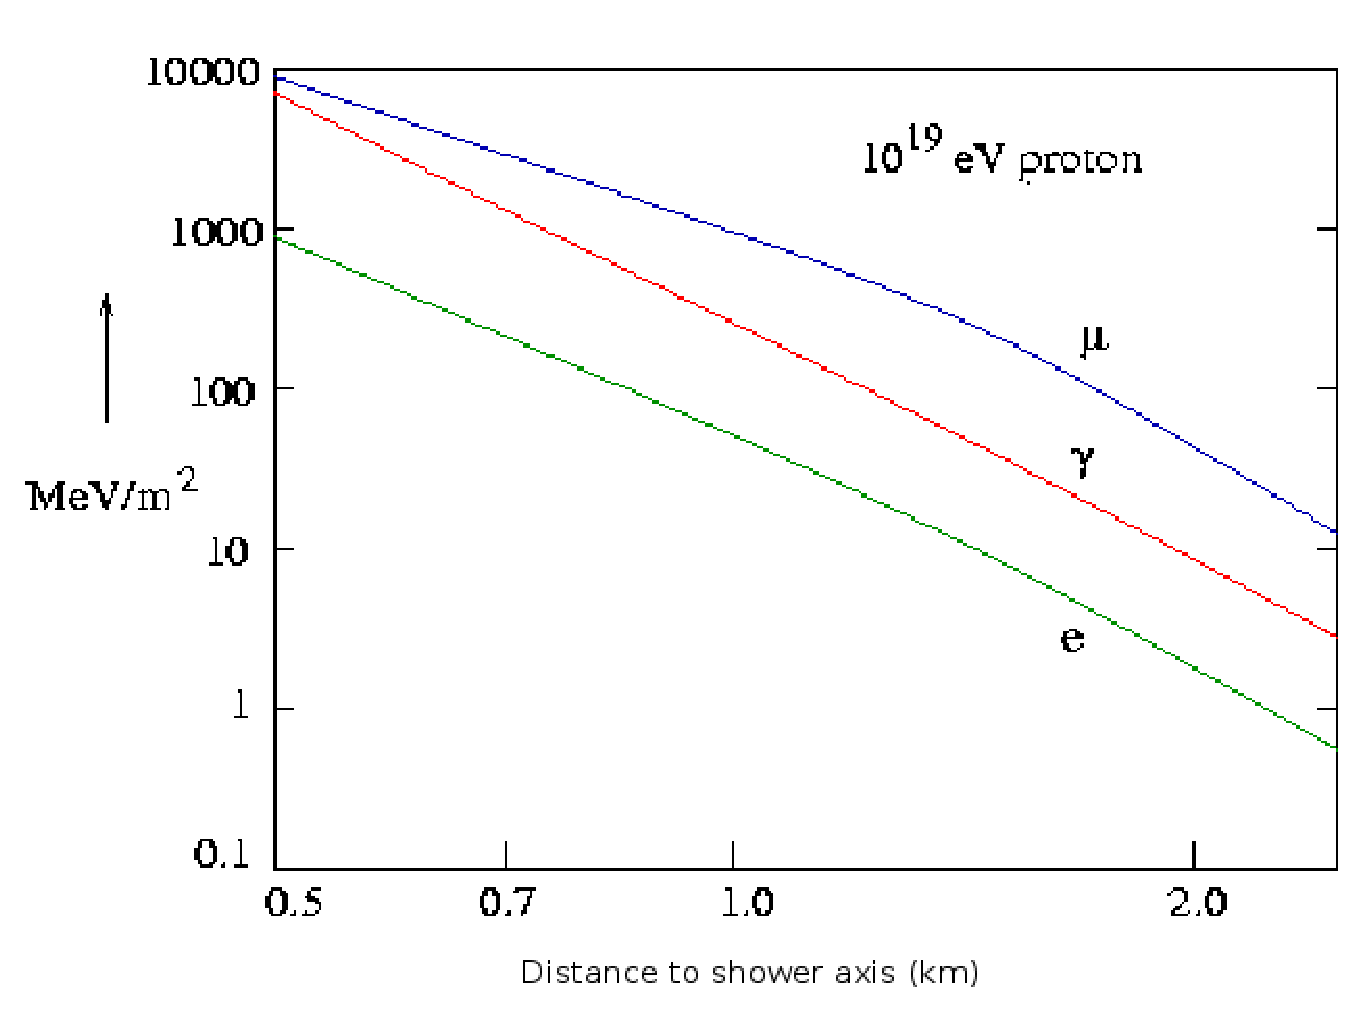
\includegraphics[scale=0.5]{profile_flux.eps}%
\caption{Energy flux of photons, electrons, and muons as a function of distance to the shower core. Simulation for a $10^{19}$~eV proton.}\label{fig:profile_flux}
\end{center}\end{figure}

The energy of the primary particle cannot be measured directly at ground level. Instead it must be estimated using the total amount of energy present in all the different components of the shower: muons, photons, electrons, and other particles not detected. It is impossible to measure every particle individually, we therefore have to make a model and assumptions.

Our first assumption is that particles lose a fixed amount of energy when passing though one gram of matter (per cm$^2$). For electrons this is 2.2~MeV per g/cm$^2$. The most important deviation of this rule of thumb is the production of new particles added to the shower. The total energy of the detectable particles can therefore be accurately estimated by determining the total number of particles and the path length of each particle. The total amount of energy lost by the particles can be calculated by adding the path lengths of all the particles and multiplying this number with the constant energy loss per unit length. To obtain the total energy in the shower we need to add the energy of the particles we did not (or could not) detect such as neutrinos and the highly energetic muons which might have penetrated a few tens or even hundreds of metres into the Earth's crust. We have to rely on simulations to obtain this energy loss, most models predict an average loss of 7\% for showers created by primary particles with an energy of $10^{19}$~eV.

In the text above we have multiple mentions of `estimation' and `model'. A small warning is appropriate. Simulations of air showers are based on extrapolations of interactions between quarks, leptons, and bosons as described by the standard model. The standard model has been extensively tested up to an energy of 200~GeV. However, the energy available at the start of an air shower is many times higher. We cannot be sure of the validity of the standard model in this energy range because we are unable to extensively test it. It might be possible that the first interactions of an air shower create quark-gluon plasmas influencing the development of the shower.

\section{HiSPARC}
How can we use the HiSPARC network and available data to reconstruct the nature, energy, and direction of the primary cosmic particles?

Scientific research into cosmic radiation makes the \emph{assumption} that all measured air showers are hadronic. A high energetic photon would create an air shower with very few muons compared to the number of electrons and muons inside an hadronic shower. This large relative shortage of muons has never been measured. This answers the first of the three questions stated at the start of this section: The shower is initiated by a charged particle. At least this is our answer until we find evidence to the contrary. The HiSPARC network will not be able to obtain this evidence because our detectors are only sensitive to muons, but this is also a preliminary assumption.

Placing a limited number of detectors across an area of 10~km$^2$ does allow us to measure the muon density at different locations inside the shower. From these measurements we can estimate the energy of the primary particle. Furthermore the distance between detectors and accurate timing of the measurements allows us to reconstruct the direction of the primary particle. For this at least three directors, roughly placed on the sides of a triangle, have to register particles. The accuracy of both calculations, energy and direction, is dependent on the number of detectors which registered the shower an the density at these detectors.

\begin{shaded}
\textbf{Exercise \theExercise \stepcounter{Exercise}} : In exercises 2 and 3 you thought about how you could estimate or calculate the energy, direction, and nature of the primary particle if one can only measure the effects at ground level. Verify your answer with the new information given in the text above and improve it if necessary.\end{shaded}

The modules `Primary Particle - Angle', `Primary Particle - Direction', and `HiSPARC detector - Detector Array' contain more information and exercises about the reconstruction of air showers.

\end{document}

